% Figure: VAE / GAN / RealNVP side by side.  Each family gets its randomness, its
% gradient and its invertibility from a different place: a reparameterised epsilon,
% a discriminator loss, or an explicit inverse with a triangular Jacobian.
% Design width ~168mm.
\documentclass[border=0pt]{standalone}
\usepackage{amsmath,amssymb}
% Shared visual language for the figures of the book.
% Every figure in this directory loads this file so the chapter reads as one system.
% NOTE: no blank lines are allowed inside \tikzset{...} (a blank line emits \par
% and breaks key scanning).
\NeedsTeXFormat{LaTeX2e}
\ProvidesPackage{figstyle}[2026/10/21 Figure style for Free Energy to LLMs]

\RequirePackage{tikz}
\usetikzlibrary{arrows.meta,positioning,calc,fit,shapes.geometric,shapes.misc,%
  backgrounds,matrix,decorations.pathreplacing,decorations.markings,patterns.meta}

% ---------------------------------------------------------------- palette
% Same values as book/preamble/style.tex, prefixed with F.
\definecolor{FNavy}{HTML}{14324A}
\definecolor{FTeal}{HTML}{0E7490}
\definecolor{FSky}{HTML}{E7F5F8}
\definecolor{FOrange}{HTML}{D97706}
\definecolor{FAmber}{HTML}{FFF3D6}
\definecolor{FInk}{HTML}{1F2937}
\definecolor{FSlate}{HTML}{64748B}
\definecolor{FMist}{HTML}{F5F7FA}
\definecolor{FRose}{HTML}{9F1239}
\definecolor{FRoseMist}{HTML}{FFF1F2}

% ---------------------------------------------------------------- semantics
% Teal   = probability / model / data object
% Orange = training objective, cost, or the quantity moved through the system
% Navy   = neutral structure
% Slate  = secondary label or metadata
% Rose   = failure mode, hazard, masked-out region
\tikzset{
  % Lay figures out in millimetres.  A figure designed 168mm wide is included at
  % \textwidth, so its fonts appear at exactly the size written here.
  every picture/.style={x=1mm,y=1mm,font=\small,line cap=round,line join=round},
  % ---- block styles
  nbase/.style={draw,rounded corners=1.2pt,align=center,inner sep=2.4pt,%
    minimum height=7mm,text=FInk},
  nteal/.style={nbase,draw=FTeal,fill=FSky},
  norange/.style={nbase,draw=FOrange,fill=FAmber},
  nnavy/.style={nbase,draw=FNavy,fill=white},
  nsoft/.style={nbase,draw=FSlate!55,fill=FMist},
  nrose/.style={nbase,draw=FRose,fill=FRoseMist},
  ghost/.style={draw=none,fill=none,align=center,inner sep=1pt},
  plain/.style={draw=none,fill=none,align=center,inner sep=0pt},
  % ---- arrows
  ar/.style={-{Latex[length=1.7mm,width=1.35mm]},draw=FSlate,line width=0.75pt},
  ard/.style={ar,dashed},
  arteal/.style={ar,draw=FTeal},
  arorange/.style={ar,draw=FOrange},
  arrose/.style={ar,draw=FRose},
  thickar/.style={ar,line width=1.2pt},
  % ---- text roles
  ftitle/.style={font=\large\bfseries,text=FNavy,align=center},
  ptitle/.style={font=\small\bfseries,text=FNavy,align=center},
  ptitleo/.style={font=\small\bfseries,text=FOrange,align=center},
  lbl/.style={font=\scriptsize,text=FSlate,align=center,inner sep=1pt},
  lblt/.style={lbl,text=FTeal},
  lblo/.style={lbl,text=FOrange},
  lbln/.style={lbl,text=FNavy},
  lblr/.style={lbl,text=FRose},
  sub/.style={font=\scriptsize,text=FSlate!90,align=center,inner sep=1pt},
  monob/.style={font=\ttfamily\scriptsize,text=FInk,inner sep=1pt},
  mathb/.style={font=\small,text=FInk,inner sep=1pt},
  eqn/.style={font=\scriptsize,inner sep=1.5pt,text=FInk},
  % ---- decorations
  brace/.style={decorate,decoration={brace,amplitude=2.4pt},draw=FSlate,%
    line width=0.6pt},
  bracet/.style={brace,draw=FTeal},
  braceo/.style={brace,draw=FOrange},
  axis/.style={draw=FSlate!55,line width=0.6pt},
  guide/.style={draw=FSlate!45,line width=0.5pt,dashed},
  halolabel/.style={font=\scriptsize,text=FInk,fill=white,fill opacity=0.85,%
    text opacity=1,inner sep=1.4pt,align=center},
}

% Figure title above the drawing, anchored at the figure's top-left.
\newcommand{\figtitle}[2][0]{%
  \node[ftitle,anchor=north west,outer sep=0pt] at (#1,0) {#2};}

% Rounded panel behind a subgroup of nodes.
\newcommand{\figpanel}[3][]{%
  \node[draw=FSlate!35,fill=#3,rounded corners=2pt,inner sep=2.6mm,#1] {#2};}

\endinput

\begin{document}
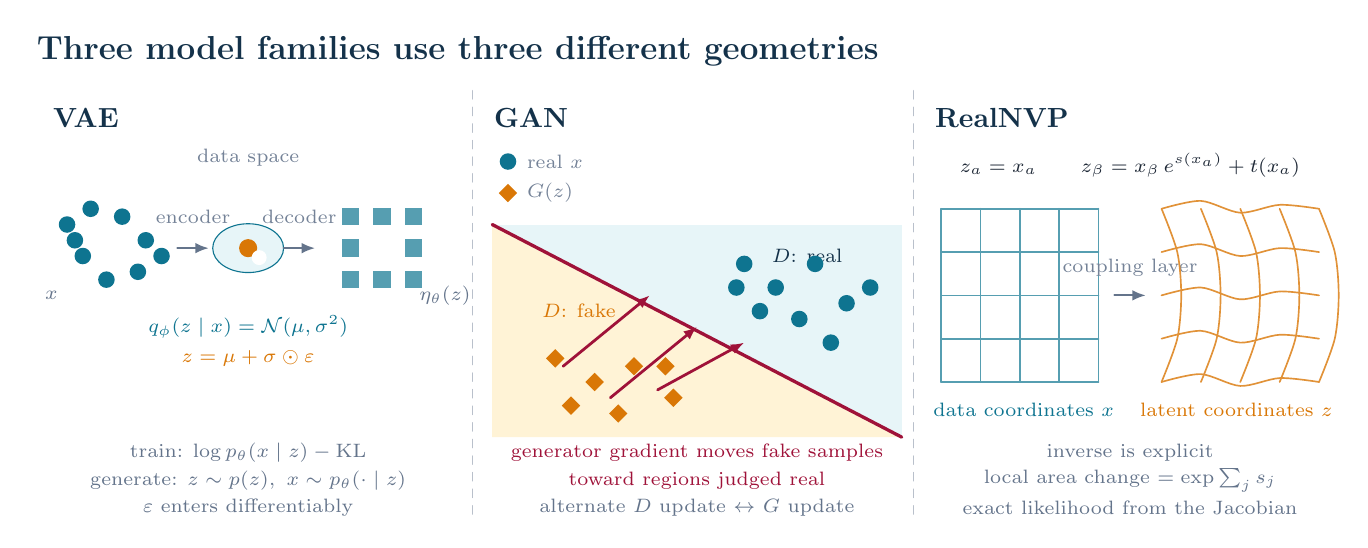
\begin{tikzpicture}
\figtitle{Three model families use three different geometries}
\node[font=\normalsize\bfseries,text=FNavy,anchor=west] at (2,-11.5) {VAE};
\node[font=\normalsize\bfseries,text=FNavy,anchor=west] at (58,-11.5) {GAN};
\node[font=\normalsize\bfseries,text=FNavy,anchor=west] at (114,-11.5) {RealNVP};
\draw[guide] (56.5,-8)--(56.5,-62);
\draw[guide] (112.5,-8)--(112.5,-62);
% ---------------------------------------------------------------------- (1) VAE
\begin{scope}[shift={(1,0)}]
\node[sub] at (27,-16.5) {data space};
\foreach \x/\y in {4/-25,7/-23,11/-24,14/-27,6/-29,9/-32,13/-31,16/-29,5/-27}
  {\fill[FTeal] (\x,\y) circle (1.05);}
\draw[ar] (18,-28)--(22,-28);
\node[sub] at (20,-24) {encoder};
\node[draw=FTeal,fill=FSky,ellipse,minimum width=9mm,minimum height=6.2mm] at (27,-28) {};
\fill[FOrange] (27,-28) circle (1.15);
\fill[white] (28.4,-29.2) circle (0.95);
\draw[ar] (31.5,-28)--(35.5,-28);
\node[sub] at (33.5,-24) {decoder};
\foreach \x/\y in {40/-24,44/-24,48/-24,40/-28,48/-28,40/-32,44/-32,48/-32}
  {\fill[FTeal!70] (\x-1.1,\y-1.1) rectangle ++(2.2,2.2);}
\node[lbl] at (2,-34) {$x$};
\node[lbl] at (52,-34) {$\eta_\theta(z)$};
\node[lblt] at (27,-38) {$q_\phi(z\mid x)=\mathcal N(\mu,\sigma^2)$};
\node[lblo] at (27,-42) {$z=\mu+\sigma\odot\varepsilon$};
\node[lbl] at (27,-54) {train: $\log p_\theta(x\mid z)-\mathrm{KL}$};
\node[lbl] at (27,-57.5) {generate: $z\sim p(z),\ x\sim p_\theta(\cdot\mid z)$};
\node[lbl] at (27,-61) {$\varepsilon$ enters differentiably};
\end{scope}
% ---------------------------------------------------------------------- (2) GAN
\begin{scope}[shift={(57,0)}]
\fill[FTeal] (4,-17) circle (1.05);
\node[sub,anchor=west] at (6,-17) {real $x$};
\node[diamond,aspect=1,fill=FOrange,draw=none,minimum size=2.4mm,inner sep=0pt] at (4,-21) {};
\node[sub,anchor=west] at (6,-21) {$G(z)$};
\fill[FSky] (2,-25) rectangle (54,-52);
\fill[FAmber] (2,-25) -- (2,-52) -- (54,-52) -- cycle;
\draw[FRose,line width=1.2pt] (2,-25)--(54,-52);
\node[lbln] at (42,-29) {$D$: real};
\node[lblo] at (13,-36) {$D$: fake};
\foreach \x/\y in {34/-30,38/-33,43/-30,47/-35,36/-36,41/-37,45/-40,50/-33,33/-33}
  {\fill[FTeal] (\x,\y) circle (1.05);}
\foreach \x/\y in {10/-42,15/-45,20/-43,25/-47,12/-48,18/-49,24/-43}
  {\node[diamond,aspect=1,fill=FOrange,draw=none,minimum size=2.4mm,inner sep=0pt] at (\x,\y) {};}
\draw[arrose,line width=1pt] (11,-43)--(22,-34);
\draw[arrose,line width=1pt] (17,-47)--(28,-38);
\draw[arrose,line width=1pt] (23,-46)--(34,-40);
\node[lblr] at (28,-54) {generator gradient moves fake samples};
\node[lblr] at (28,-57.5) {toward regions judged real};
\node[lbl] at (28,-61) {alternate $D$ update $\leftrightarrow$ $G$ update};
\end{scope}
% ------------------------------------------------------------------ (3) RealNVP
\begin{scope}[shift={(113,0)}]
\node[eqn] at (27,-17.5) {$z_a=x_a \qquad z_\beta=x_\beta\,e^{s(x_a)}+t(x_a)$};
\foreach \x in {3,8,13,18,23}
  {\draw[draw=FTeal!70,line width=0.6pt] (\x,-23)--(\x,-45);}
\foreach \y in {-23,-28.5,-34,-39.5,-45}
  {\draw[draw=FTeal!70,line width=0.6pt] (3,\y)--(23,\y);}
\draw[ar] (25,-34)--(29,-34);
\node[sub] at (27,-30.5) {coupling layer};
\draw[draw=FOrange!80,line width=0.6pt,smooth] plot coordinates
  {(31,-23)(33,-28.5)(33.5,-34)(33,-39.5)(31,-45)};
\draw[draw=FOrange!80,line width=0.6pt,smooth] plot coordinates
  {(36,-23)(38,-28.5)(38.5,-34)(38,-39.5)(36,-45)};
\draw[draw=FOrange!80,line width=0.6pt,smooth] plot coordinates
  {(41,-23)(43,-28.5)(43.5,-34)(43,-39.5)(41,-45)};
\draw[draw=FOrange!80,line width=0.6pt,smooth] plot coordinates
  {(46,-23)(48,-28.5)(48.5,-34)(48,-39.5)(46,-45)};
\draw[draw=FOrange!80,line width=0.6pt,smooth] plot coordinates
  {(51,-23)(53,-28.5)(53.5,-34)(53,-39.5)(51,-45)};
\draw[draw=FOrange!80,line width=0.6pt,smooth] plot coordinates
  {(31,-23)(36,-22)(41,-23.5)(46,-22.5)(51,-23)};
\draw[draw=FOrange!80,line width=0.6pt,smooth] plot coordinates
  {(31,-28.5)(36,-27.5)(41,-29)(46,-28)(51,-28.5)};
\draw[draw=FOrange!80,line width=0.6pt,smooth] plot coordinates
  {(31,-34)(36,-33)(41,-34.5)(46,-33.5)(51,-34)};
\draw[draw=FOrange!80,line width=0.6pt,smooth] plot coordinates
  {(31,-39.5)(36,-38.5)(41,-40)(46,-39)(51,-39.5)};
\draw[draw=FOrange!80,line width=0.6pt,smooth] plot coordinates
  {(31,-45)(36,-44)(41,-45.5)(46,-44.5)(51,-45)};
\node[lblt] at (13.5,-48.5) {data coordinates $x$};
\node[lblo] at (40.5,-48.5) {latent coordinates $z$};
\node[lbl] at (27,-54) {inverse is explicit};
\node[lbl] at (27,-57.5) {local area change $=\exp\sum_j s_j$};
\node[lbl] at (27,-61) {exact likelihood from the Jacobian};
\end{scope}
\end{tikzpicture}
\end{document}
